\documentclass[aspectratio=43]{beamer}

% Text packages to stop warnings
\usepackage{lmodern}
\usepackage{textcomp}
\usepackage{listings}
\usepackage{multirow}
\usepackage{tikz}

\usetikzlibrary{arrows,automata,shapes,positioning}
\tikzstyle{block} = [rectangle, draw, fill=blue!20, 
    text width=2.5em, text centered, rounded corners, minimum height=2em]
\tikzstyle{bw} = [rectangle, draw, fill=blue!20, 
    text width=3.5em, text centered, rounded corners, minimum height=2em]

% Themes
\usetheme{Boadilla}
\setbeamertemplate{footline}[page number]{}
\setbeamertemplate{navigation symbols}{}

% Suppress the navigation bar
\beamertemplatenavigationsymbolsempty

\lstset{basicstyle=\scriptsize, frame=single}

\newenvironment{changemargin}[1]{% 
  \begin{list}{}{% 
    \setlength{\topsep}{0pt}% 
    \setlength{\leftmargin}{#1}% 
    \setlength{\rightmargin}{1em}
    \setlength{\listparindent}{\parindent}% 
    \setlength{\itemindent}{\parindent}% 
    \setlength{\parsep}{\parskip}% 
  }% 
  \item[]}{\end{list}} 

\title{Lecture 14---Parallelization: Patterns and Strategy}
\subtitle{ECE 459: Programming for Performance}
\date{February 4, 2015}

\begin{document}

%%%%%%%%%%%%%%%%%%%%%%%%%%%%%%%%%%%%%%%%%%%%%%%%%%%%%%%%%%%%%%%%%%%%%%%%%%%%%%%%
\begin{frame}[plain]
  \titlepage
\end{frame}
%%%%%%%%%%%%%%%%%%%%%%%%%%%%%%%%%%%%%%%%%%%%%%%%%%%%%%%%%%%%%%%%%%%%%%%%%%%%%%%%


%%%%%%%%%%%%%%%%%%%%%%%%%%%%%%%%%%%%%%%%%%%%%%%%%%%%%%%%%%%%%%%%%%%%%%%%%%%%%%%%
\begin{frame}
  \frametitle{Assignment 2 Preview}

\large
  \begin{changemargin}{1.5cm}
  Three parts:
  \begin{enumerate}
    \item Restructuring code for Automatic Parallelization.
    \item Manual parallelization of a loop with OpenMP.
    \item Using OpenMP tasks effectively.
  \end{enumerate}

  \end{changemargin}
\end{frame}
%%%%%%%%%%%%%%%%%%%%%%%%%%%%%%%%%%%%%%%%%%%%%%%%%%%%%%%%%%%%%%%%%%%%%%%%%%%%%%%%

\part{More Parallelization Patterns}
\frame{\partpage}

%%%%%%%%%%%%%%%%%%%%%%%%%%%%%%%%%%%%%%%%%%%%%%%%%%%%%%%%%%%%%%%%%%%%%%%%%%%%%%%%
\begin{frame}
  \frametitle{Pattern 5: Pipeline of Tasks}

  \begin{changemargin}{2.5cm}
    Seen briefly in computer architecture.

    \begin{itemize}
    \item Use multiple stages; each thread handles a stage.\\[1em]
     {\bf Example:} a program that handles network packets: (1) accepts
      packets, (2) processes them, and (3) re-transmits them. Could set up the threads such that each packet goes through the threads.
    \vfill
    \item Improves \structure{throughput}; may increase \structure{latency} as
      there's communication between threads.
    \vfill
    \item In the best case, you'll have a linear speedup.\\[1em]

     Rare, since the runtime of the stages will vary, and the slow
      one will be the bottleneck (but you could have 2 instances of the
      slow stage).
  \end{itemize}
  \end{changemargin}
\end{frame}
%%%%%%%%%%%%%%%%%%%%%%%%%%%%%%%%%%%%%%%%%%%%%%%%%%%%%%%%%%%%%%%%%%%%%%%%%%%%%%%%

%%%%%%%%%%%%%%%%%%%%%%%%%%%%%%%%%%%%%%%%%%%%%%%%%%%%%%%%%%%%%%%%%%%%%%%%%%%%%%%%
\begin{frame}
  \frametitle{Pattern 6: Client-Server}

  \begin{changemargin}{2.5cm}
    To execute a large computation, the server supplies work to many
      clients---as many as request it.\\[1em]

    Client computes results and returns them to the server.\\[1em]
   {\bf Examples:} botnets, {\tt SETI@Home}, GUI application (backend
      acts as the server).\\[1em]
   Server can arbitrate access to shared resources (such as network
      access) by storing the requests and sending them out.\\[1em]

   \begin{itemize}
    \item Parallelism is somewhere between single task, multiple threads and
      multiple loosely-coupled tasks  
  \end{itemize}
  \end{changemargin}
\end{frame}
%%%%%%%%%%%%%%%%%%%%%%%%%%%%%%%%%%%%%%%%%%%%%%%%%%%%%%%%%%%%%%%%%%%%%%%%%%%%%%%%

%%%%%%%%%%%%%%%%%%%%%%%%%%%%%%%%%%%%%%%%%%%%%%%%%%%%%%%%%%%%%%%%%%%%%%%%%%%%%%%%
\begin{frame}
  \frametitle{Pattern 7: Producer-Consumer}

  \begin{changemargin}{2.5cm}
    Variant on the pipeline and client-server models.\\
    Producer generates work, and consumer performs work.\\[1em]
    {\bf Example:} producer which generates rendered frames;
      consumer which orders these frames and writes them to disk.\\[1em]
    Any number of producers and consumers.\\[1em]

    \begin{itemize}
    \item This approach can improve \structure{throughput} and also reduces
      design complexity
    \end{itemize}
  \end{changemargin}
\end{frame}
%%%%%%%%%%%%%%%%%%%%%%%%%%%%%%%%%%%%%%%%%%%%%%%%%%%%%%%%%%%%%%%%%%%%%%%%%%%%%%%%

%%%%%%%%%%%%%%%%%%%%%%%%%%%%%%%%%%%%%%%%%%%%%%%%%%%%%%%%%%%%%%%%%%%%%%%%%%%%%%%%
\begin{frame}
  \frametitle{Combining Strategies}

  \begin{changemargin}{2.5cm}
    Most problems don't fit into one category, so it's often best to combine
      strategies.\\[1em]

    For instance, you might often start with a pipeline, and then use
      multiple threads in a particular pipeline stage to handle one piece of
      data.\\[1em]
    Tip: estimate to see what divisions of strategies would work best
      (might have to do more iterations of Amdahl's law depending on the amount
      of strategies you can use).
  \end{changemargin}

\end{frame}
%%%%%%%%%%%%%%%%%%%%%%%%%%%%%%%%%%%%%%%%%%%%%%%%%%%%%%%%%%%%%%%%%%%%%%%%%%%%%%%%

%%%%%%%%%%%%%%%%%%%%%%%%%%%%%%%%%%%%%%%%%%%%%%%%%%%%%%%%%%%%%%%%%%%%%%%%%%%%%%%%
\begin{frame}
  \frametitle{Midterm Questions from 2011 (1)}

\begin{changemargin}{2.5cm}
  For each of the following situations, {\bf name an appropriate parallelization
  pattern and the granularity at which you would apply it, explain the necessary
  communication, and explain why your pattern is appropriate}.
  \begin{itemize}
  \item build system, e.g. parallel make
    \begin{itemize}
      \item<2-> Multiple independent tasks, at a per-file granularity
    \end{itemize}
  \item optical character recognition system
    \begin{itemize}
      \item<2-> Pipeline of tasks
      \item<2-> 2 tasks - finding characters and analyzing them
    \end{itemize}
  \end{itemize}
\end{changemargin}
\end{frame}
%%%%%%%%%%%%%%%%%%%%%%%%%%%%%%%%%%%%%%%%%%%%%%%%%%%%%%%%%%%%%%%%%%%%%%%%%%%%%%%%

%%%%%%%%%%%%%%%%%%%%%%%%%%%%%%%%%%%%%%%%%%%%%%%%%%%%%%%%%%%%%%%%%%%%%%%%%%%%%%%%
\begin{frame}
  \frametitle{Midterm Questions from 2011 (2)}

\begin{changemargin}{2.5cm}
  {\bf Give a concrete example} where you would use the following
  parallelization patterns. {\bf Explain} the granularity at which you'd apply
  the pattern.
  \begin{itemize}
    \item single task, multiple threads:
    \begin{itemize}
      \item<2-> Computation of a mathematical function with independent
        sub-formulas.
    \end{itemize}
    \item producer-consumer (no rendering frames, please):
    \begin{itemize}
      \item<2-> Processing of stock-market data:
        a server might generate raw financial data (quotes) for a
        particular security. The server would be the producer. Several clients
        (or consumers) may take the raw data and use them in different ways, e.g. by computing means, generating charts, etc.
    \end{itemize}
  \end{itemize}
 \end{changemargin}
\end{frame}
%%%%%%%%%%%%%%%%%%%%%%%%%%%%%%%%%%%%%%%%%%%%%%%%%%%%%%%%%%%%%%%%%%%%%%%%%%%%%%%%

%%%%%%%%%%%%%%%%%%%%%%%%%%%%%%%%%%%%%%%%%%%%%%%%%%%%%%%%%%%%%%%%%%%%%%%%%%%%%%%%
\part{Parallelizing Code}
\frame{\partpage}

%%%%%%%%%%%%%%%%%%%%%%%%%%%%%%%%%%%%%%%%%%%%%%%%%%%%%%%%%%%%%%%%%%%%%%%%%%%%%%%%
\begin{frame}
  \frametitle{How To Parallelize Code: Strategy}
  
  \begin{changemargin}{2.5cm}
  Four-step outline:
  \begin{enumerate}
    \item Profile the code.
    \item Look at hotspots; find and optimize dependencies; parallelize dependency chains; change the algorithm if you can.
    \item Estimate benefits.
    \item If not good enough, step back and try higher level of abstraction.
  \end{enumerate}
  Always try to minimize synchronization.
  \end{changemargin}

\end{frame}
%%%%%%%%%%%%%%%%%%%%%%%%%%%%%%%%%%%%%%%%%%%%%%%%%%%%%%%%%%%%%%%%%%%%%%%%%%%%%%%%


%%%%%%%%%%%%%%%%%%%%%%%%%%%%%%%%%%%%%%%%%%%%%%%%%%%%%%%%%%%%%%%%%%%%%%%%%%%%%%%%
\begin{frame}
  \frametitle{Low-level Implementation Tactic: Thread Pools}
  
  \begin{changemargin}{2.5cm}
    Instead of creating threads, destroying them and recreating them, you
      can use a \structure{thread pool}.
    \begin{itemize}
    \item It creates $n$ threads; you just {\tt push} work onto them.
    \end{itemize}

  \begin{center}
    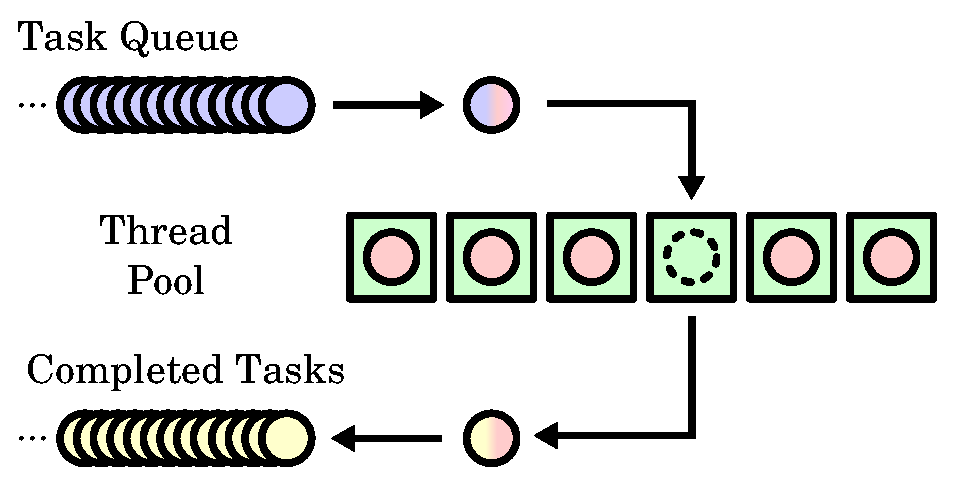
\includegraphics[scale=0.4]{L14/thread-pool}
  \end{center}

  \begin{itemize}
    \item Only question is: How many threads should you create? (Experiment to find out).
    \item Implementation from GLib: {\tt GThreadPool}.
  \end{itemize}
  \end{changemargin}

\end{frame}
%%%%%%%%%%%%%%%%%%%%%%%%%%%%%%%%%%%%%%%%%%%%%%%%%%%%%%%%%%%%%%%%%%%%%%%%%%%%%%%%


%%%%%%%%%%%%%%%%%%%%%%%%%%%%%%%%%%%%%%%%%%%%%%%%%%%%%%%%%%%%%%%%%%%%%%%%%%%%%%%%
\begin{frame}
  \frametitle{Introduction to Automatic Parallelization}

  \begin{changemargin}{2.5cm}
    Vision: take a sequential C program and \\ automatically convert it into a parallel version.\\[1em]

    Lots of research in the early 1990s, then tapered off.\\~~~(it's hard!)\\[1em]

    Renewed interest now since multicores are so common.\\~~~(it's still hard!)
  \end{changemargin}
\end{frame}
%%%%%%%%%%%%%%%%%%%%%%%%%%%%%%%%%%%%%%%%%%%%%%%%%%%%%%%%%%%%%%%%%%%%%%%%%%%%%%%%

%%%%%%%%%%%%%%%%%%%%%%%%%%%%%%%%%%%%%%%%%%%%%%%%%%%%%%%%%%%%%%%%%%%%%%%%%%%%%%%%
\begin{frame}
  \frametitle{What Can We Parallelize?}

  \begin{changemargin}{2.5cm}
  
  \begin{itemize}
    \item Some languages are easier than others to reason about (and therefore to
      automatically parallelize).
    \item C can be easy to parallelize, given the right code, plus compiler hints.
    \item ``The right code'' = arrays with no loop-carried dependencies.
  \end{itemize}
  \end{changemargin}
\end{frame}

%%%%%%%%%%%%%%%%%%%%%%%%%%%%%%%%%%%%%%%%%%%%%%%%%%%%%%%%%%%%%%%%%%%%%%%%%%%%%%%%
\begin{frame}
  \frametitle{Automatic Parallelization in Practice}
  \begin{changemargin}{2cm}
    Some production compilers support automatic parallelization: 
    \begin{itemize}
      \item {\tt icc} (Intel's
      non-free compiler);
      \item {\tt solarisstudio} (Oracle's free-as-in-beer
      compiler \footnote{\tiny \url{http://www.oracle.com/technetwork/documentation/solaris-studio-12-192994.html}});
      \item {\tt gcc} (GNU's free-as-in-speech compiler).
    \end{itemize}
  \end{changemargin}

\end{frame}
%%%%%%%%%%%%%%%%%%%%%%%%%%%%%%%%%%%%%%%%%%%%%%%%%%%%%%%%%%%%%%%%%%%%%%%%%%%%%%%%

%%%%%%%%%%%%%%%%%%%%%%%%%%%%%%%%%%%%%%%%%%%%%%%%%%%%%%%%%%%%%%%%%%%%%%%%%%%%%%%%
\begin{frame}[fragile]
  \frametitle{Example Code from the Textbook}

  \begin{changemargin}{1.5cm}
    We saw automatic parallelization of some code.\\
    Let's revisit the whole issue in Lecture 16.
  \end{changemargin}
  
\end{frame}
%%%%%%%%%%%%%%%%%%%%%%%%%%%%%%%%%%%%%%%%%%%%%%%%%%%%%%%%%%%%%%%%%%%%%%%%%%%%%%%%

%%%%%%%%%%%%%%%%%%%%%%%%%%%%%%%%%%%%%%%%%%%%%%%%%%%%%%%%%%%%%%%%%%%%%%%%%%%%%%%%
\part{Parallelizing Code}
\frame{\partpage}

%%%%%%%%%%%%%%%%%%%%%%%%%%%%%%%%%%%%%%%%%%%%%%%%%%%%%%%%%%%%%%%%%%%%%%%%%%%%%%%%
\begin{frame}[fragile]
  \frametitle{Example Code from the Textbook}

\begin{changemargin}{1.5cm}
Following Gove, we'll parallelize the following code:

  \begin{lstlisting}[numbers=left]
#include <stdlib.h>

void setup(double *vector, int length) {
    int i;
    for (i = 0; i < length; i++)
    {
        vector[i] += 1.0;
    }
}

int main()
{
    double *vector;
    vector = (double*) malloc(sizeof(double)*1024*1024);
    for (int i = 0; i < 1000; i++)
    {
        setup (vector, 1024*1024);
    }
}
  \end{lstlisting}
\end{changemargin}
\end{frame}
%%%%%%%%%%%%%%%%%%%%%%%%%%%%%%%%%%%%%%%%%%%%%%%%%%%%%%%%%%%%%%%%%%%%%%%%%%%%%%%%

%%%%%%%%%%%%%%%%%%%%%%%%%%%%%%%%%%%%%%%%%%%%%%%%%%%%%%%%%%%%%%%%%%%%%%%%%%%%%%%%
\begin{frame}[fragile]
  \frametitle{Automatic Parallelization of Example Code}

\begin{changemargin}{1.5cm}
  Let's try automatic parallelization.
  \vfill
  Compiling with {\tt solarisstudio} and automatic parallelization yields
  the following:
\end{changemargin}

{\scriptsize
  \begin{lstlisting}
% solarisstudio-cc -O3 -xautopar -xloopinfo omp_vector.c 
"omp_vector.c", line 5: PARALLELIZED, and serial version generated                 
"omp_vector.c", line 15: not parallelized, call may be unsafe
  \end{lstlisting}
}
\begin{changemargin}{1.5cm}
  How will this code compare to our manual efforts? \\
  (If you weren't in class, you'll have to try it yourself.)
  \vfill
  {\bf Note:} {\tt solarisstudio} generates two versions of the code, 
  and decides, at runtime, if the parallel code would be faster.
\end{changemargin}

\end{frame}
%%%%%%%%%%%%%%%%%%%%%%%%%%%%%%%%%%%%%%%%%%%%%%%%%%%%%%%%%%%%%%%%%%%%%%%%%%%%%%%%


\end{document}
